\documentclass[
  xcolor={svgnames},
  hyperref={colorlinks,citecolor=DeepPink4,linkcolor=DarkRed,urlcolor=DarkBlue}
  ]{beamer}  % for hardcopy add 'trans'

\usetheme{Boadilla}
% \usepackage{beamerthemesplit} // Activate for custom appearance

%\usepackage{paralist}
%\usepackage{enumerate}
\setbeamertemplate{caption}[numbered]

\setbeamercolor{item projected}{bg=blue}
\setbeamertemplate{enumerate items}[default]
\setbeamertemplate{navigation symbols}{}
\setbeamercovered{transparent}
\setbeamercolor{block title}{fg=blue}
\setbeamercolor{local structure}{fg=blue}
\setbeamercolor{caption name}{fg=blue}

\usepackage{transparent}
% \usepackage{tikz}
% \usepackage{CJKutf8}
% \usetikzlibrary{shapes}

% \newcommand{\semitransp}[2][35]{\color{fg!#1}#2}

%%%%%%%%%%%%%%%%%%%%%%%%%%%%%%%%%%%%%%%%%%%%%%%%%%%%%%%%%%%%%%%%%%%%%%%%%%%%%%%%%%%
%% Load packages
%%%%%%%%%%%%%%%%%%%%%%%%%%%%%%%%%%%%%%%%%%%%%%%%%%%%%%%%%%%%%%%%%%%%%%%%%%%%%%%%%%%

\usepackage{fancybox}
% \usepackage{enumitem} % Has to do with enumeration
\usepackage{amsfonts}
\usepackage{amsmath}
\usepackage{amsthm} % Allows for labeling of theorems
\usepackage[T1]{fontenc}
\usepackage[utf8]{inputenc}
\usepackage{graphicx}
\graphicspath{ {Figures/} }
\usepackage{hyperref}
\hypersetup{
    colorlinks,
    citecolor=black,
    filecolor=black,
    linkcolor=blue,
    urlcolor=blue
}
\newtheorem{thm}{Theorem}[section]
\newtheorem{lem}[thm]{Lemma}
\newtheorem{prop}[thm]{Proposition}
\newtheorem{cor}[thm]{Corollary}
% \usepackage{appendix}
% \usepackage{subfigure} % For plotting multiple figures at once
% \usepackage{verbatim}  % for including verbatim code from a file
% \usepackage{pdfpages}

\usepackage{textcomp} % to get upquotes in listings environments.
\usepackage{listings} % for texing code
%\usepackage{alltt}
%\usepackage{courier}
\usepackage{xcolor}

%%%%%%%%%%%%%%%%%%%%%%%%%%%%%%%%%%%%%%%%%%%%%%%%%%%%%%%%%%%%%%%%%%%%%%%%%%%%%%%%%%%
%% Colors
%%%%%%%%%%%%%%%%%%%%%%%%%%%%%%%%%%%%%%%%%%%%%%%%%%%%%%%%%%%%%%%%%%%%%%%%%%%%%%%%%%%

\definecolor{codegreen}{RGB}{28,172,0}
\definecolor{codelilas}{RGB}{170,55,241}
\definecolor{gray}{RGB}{120,120,120}
\definecolor{LightGray}{gray}{.85}

\newcommand\boldblue[1]{\textcolor{blue}{\textbf{#1}}}

%%%%%%%%%%%%%%%%%%%%%%%%%%%%%%%%%%%%%%%%%%%%%%%%%%%%%%%%%%%%%%%%%%%%%%%%%%%%%%%%%%%
%% Configure TeXed code
%%%%%%%%%%%%%%%%%%%%%%%%%%%%%%%%%%%%%%%%%%%%%%%%%%%%%%%%%%%%%%%%%%%%%%%%%%%%%%%%%%%

%% Bash
\lstdefinestyle{bash}{%
  language=bash,%
  basicstyle=\footnotesize\ttfamily,%
  showstringspaces=false,%
  commentstyle=\color{gray},%
  keywordstyle=\color{blue},%
  xleftmargin=0.25in,%
  xrightmargin=0.25in,%
  upquote=true
}
\newcommand\bashstyle{\lstset{style=bash}}

%% MATLAB
\lstdefinestyle{matlab}{%
  language=Matlab,%
  basicstyle=\footnotesize\ttfamily,%
  breaklines=true,%
  morekeywords={matlab2tikz},%
  keywordstyle=\color{blue},%
  morekeywords=[2]{1}, keywordstyle=[2]{\color{black}},%
  identifierstyle=\color{black},%
  stringstyle=\color{codelilas},%
  commentstyle=\color{codegreen},%
  showstringspaces=false,%
    %   Without this there will be a symbol in
    %   the places where there is a space
  emph=[1]{for,end,break,switch,case},emphstyle=[1]\color{blue},%
    %   Some words to emphasise
  upquote=true
}
\newcommand\matlabstyle{\lstset{style=matlab}}

\newcommand{\matlabcode}[1]{%
    \matlabstyle%
    \lstinputlisting{#1}
}

%% Julia

% Highlight the 'julia>' prompt.
% See http://tex.stackexchange.com/a/172076/50294 for the additional highlighting
% See http://tex.stackexchange.com/a/180619/50294 for the '>' issue
\makeatletter
\lst@InstallKeywords k{attributes}{attributestyle}\slshape{attributestyle}{}ld
\makeatother

% (c) 2014 Jubobs
% See http://tex.stackexchange.com/a/212794
\lstdefinelanguage{Julia}%
{morekeywords={abstract,break,case,catch,const,continue,do,else,elseif,%
    end,export,false,for,function,immutable,import,importall,if,in,%
    macro,module,otherwise,quote,return,switch,true,try,type,typealias,%
    using,while},%
  sensitive=true,%
  alsoother={\$},%
  morecomment=[l]\#,%
  morecomment=[n]{\#=}{=\#},%
  morestring=[s]{"}{"},%
  morestring=[m]{'}{'},%
}[keywords,comments,strings]%


\lstdefinestyle{julia}{%
  language=Julia,%
  basicstyle=\footnotesize\ttfamily,%
  breaklines=true,%
  keywordstyle=\bfseries\color{blue},%
  identifierstyle=\color{black},%
  stringstyle=\color{codegreen},%
  commentstyle=\color{codelilas},%
  showstringspaces=false,%
  upquote=true,%
  backgroundcolor=\color{LightGray},%
  alsoletter={>},%
  moreattributes={julia>}, %
  attributestyle = \bfseries\color{green}, %
  escapeinside={\%*}{*)},          % if you want to add LaTeX within your code
}
\newcommand\juliastyle{\lstset{style=julia}}

\newcommand{\juliacode}[1]{%
    \juliastyle%
    \lstinputlisting{#1}
}


% Set up in-line code snippets.
% See http://tex.stackexchange.com/a/42964 and
%     http://tex.stackexchange.com/a/83883/50294
\newcommand\bashinline[1]{\colorbox{LightGray}{{\bashstyle\lstinline!#1!}}}
\newcommand\matlabinline[1]{\colorbox{LightGray}{{\matlabstyle\lstinline!#1!}}}
\newcommand\juliainline[1]{\colorbox{LightGray}{{\juliastyle\lstinline!#1!}}}
\newcommand\genericinline[1]{\colorbox{LightGray}{#1}}


\title{Macroeconomic Modeling with Julia}
\author{Pearl Li}
\institute[New York Fed]{Federal Reserve Bank of New York}
\date{December 18, 2017}

\begin{document}
\maketitle

\section{Intro}
\begin{frame}
  \frametitle{Thank yous}

  \begin{itemize}
    \setlength\itemsep{1em}
    \item Cristina Griffa and workshop organizers
    \item DSGE team at the New York Fed
    \item John Stachurski, for much of the content on these slides
    \item You all for being here
  \end{itemize}
\end{frame}

\begin{frame}
  \frametitle{Team}

  \begin{itemize}
    \setlength\itemsep{1em}
    \item \boldblue{Abhi Gupta}: Senior Research Analyst at New York Fed
    \item \boldblue{Pearl Li }: Senior Research Analyst at New York Fed
  \end{itemize}
\end{frame}

\begin{frame}
  \frametitle{Goals and Assumptions}

  \vspace{1em}

  \boldblue{Assumptions}
  \begin{itemize}
    \item Attendees are programmers but new to Julia
    \item Interested in macroeconomics
  \end{itemize}

  \vspace{1em}

  \boldblue{Goals}
  \begin{itemize}
    \item Overview of Julia and comparisons to other languages
    \item Lower fixed costs to learning Julia
    \item Resources for further study
  \end{itemize}

\end{frame}

\begin{frame}
  \frametitle{Schedule}

  \boldblue{Day 1}
  %
  \begin{itemize}
    \item Introduction to Julia (Pearl)
    \item Julia syntax (Abhi)
    \item Types and multiple dispatch (Pearl)
  \end{itemize}

  \vspace{1em}
  \boldblue{Day 2}
  %
  \begin{itemize}
    \item Julia for economists -- packages and libraries (Abhi)
    \item State-space routines (Abhi) and DSGE.jl (Pearl)
  \end{itemize}
\end{frame}


\begin{frame}
  \frametitle{Resources}

  \begin{center}
  \href{http://github.com/FRBNY-DSGE/IADB\_2017\_Workshop}{http://github.com/FRBNY-DSGE/IADB\_2017\_Workshop}
  \end{center}
  \vspace{2em}

  More resources listed there.
\end{frame}


\begin{frame}
  \frametitle{Software Options}

  Install
  \begin{itemize}
    \item Julia
    \item Packages (IJulia, QuantEcon.jl, DSGE.jl)
    \item IDE if you like (such as Juno)
  \end{itemize}

  \vspace{1em}
  Or
  \begin{itemize}
    \item JuliaPro
  \end{itemize}

  \vspace{1em}
  Or don't install
  \begin{itemize}
    \item JuliaBox (\href{juliabox.org}{juliabox.org}) TODO
  \end{itemize}

\end{frame}

\section{Overview}

\begin{frame}
  \frametitle{Scientific Computing}

  Using computation to solve scientific/engineering problems.

  \vspace{1em}
  \boldblue{Tasks:}
  \begin{itemize}
    \item Solve numerical problems
    \item Manipulate data
    \item Simulate
    \item Visualize results with tables and graphs
    \item Explore
  \end{itemize}

  \pause
  \vspace{1em}
  And we often want to do these things \boldblue{fast}.
\end{frame}

\begin{frame}
  \frametitle{Speed is nontrivial}

  To get maximum speed, we need:
  \begin{itemize}
    \item Optimal use of hardware
    \item High level of control over operations/logic
  \end{itemize}

  \vspace{1em}
  First best: \boldblue{assembly language}/machine code. This gives us
  instructions at the CPU level, specific to your chip architecture.

  \vspace{1em}
  For example: $1 + 2$

\end{frame}

\begin{frame}[fragile]
  \frametitle{$1 + 2$}

  \lstset{style=julia}
  \begin{lstlisting}
    .cfi_startproc
    pushq %rbp
    .cfi_def_cfa_offset 16
    .cfi_offset 6, -16
    movq %rsp, %rbp
    .cfi_def_cfa_register 6
    movl $1, -12(%rbp)
    movl $2, -8(%rbp)
    movl -12(%rbp), %edx
    movl -8(%rbp), %eax
    addl %edx, %eax
    movl %eax, -4(%rbp)
    movl -4(%rbp), %eax
    popq %rbp
    .cfi_def_cfa 7, 8
    ret
    .cfi_endproc
  \end{lstlisting}

\end{frame}

\begin{frame}
  Now imagine programming a 3-equation DSGE model like this... \\

  \vspace{1em}
  You would have to optimize for specific hardware:
  \begin{itemize}
    \item Pipelining
    \item Cache hierarchies
    \item Branch prediction
    \item Multiprocessing
    \item etc, etc, etc
  \end{itemize}

  \vspace{1em}
  \pause
  And change it every time there's a new processor.

\end{frame}

\begin{frame}
  \frametitle{Tradeoffs}

  \boldblue{Low level languages} give us:
  \begin{itemize}
    \item Speed
    \item Fine-grained control
    \item Less machine time, more programmer time
  \end{itemize}

  \pause

  \vspace{1em}
  \boldblue{High level languages} give us:
  \begin{itemize}
    \item Abstraction (from hardware, pointers, etc)
    \item Automation of some tasks (garbage collection)
    \item Natural language representations
    \item Less programmer time, more machine time
  \end{itemize}

\end{frame}

\begin{frame}

  \begin{figure}
    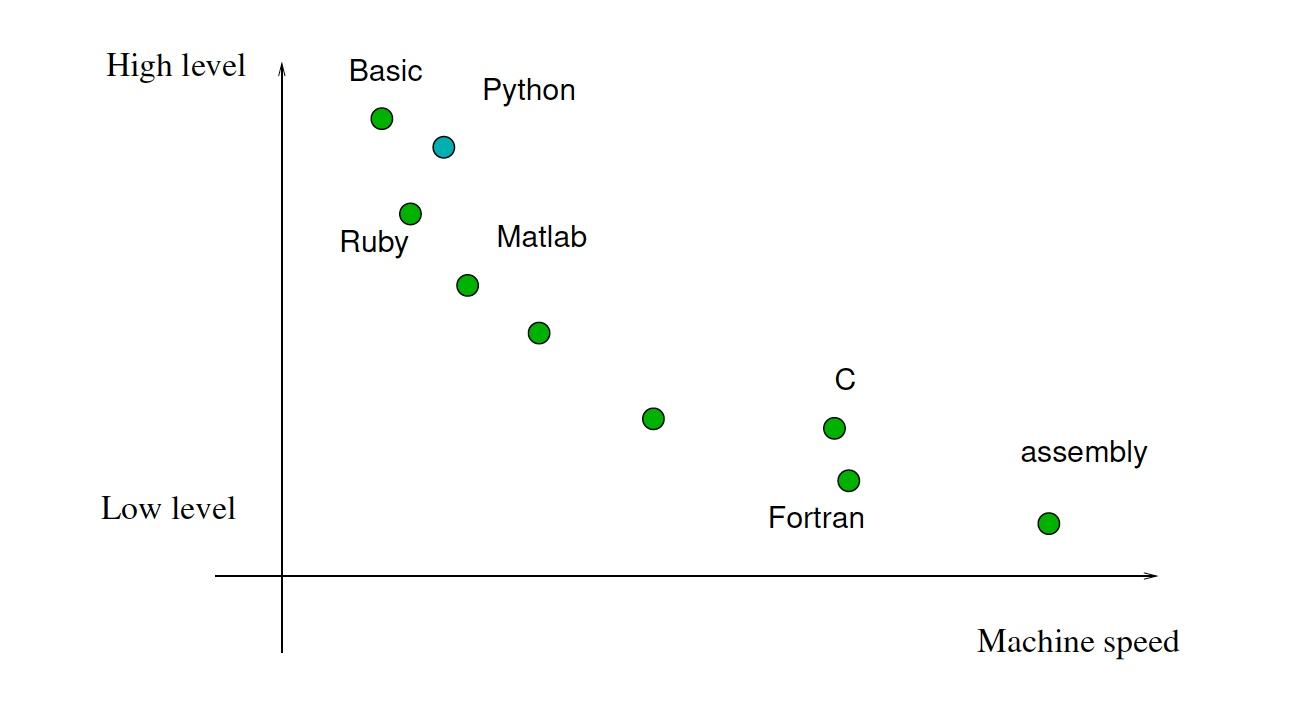
\includegraphics[width=\textwidth]{languages.jpeg}
  \end{figure}

  But the curve is starting to shift...
\end{frame}

\begin{frame}

  \begin{figure}
    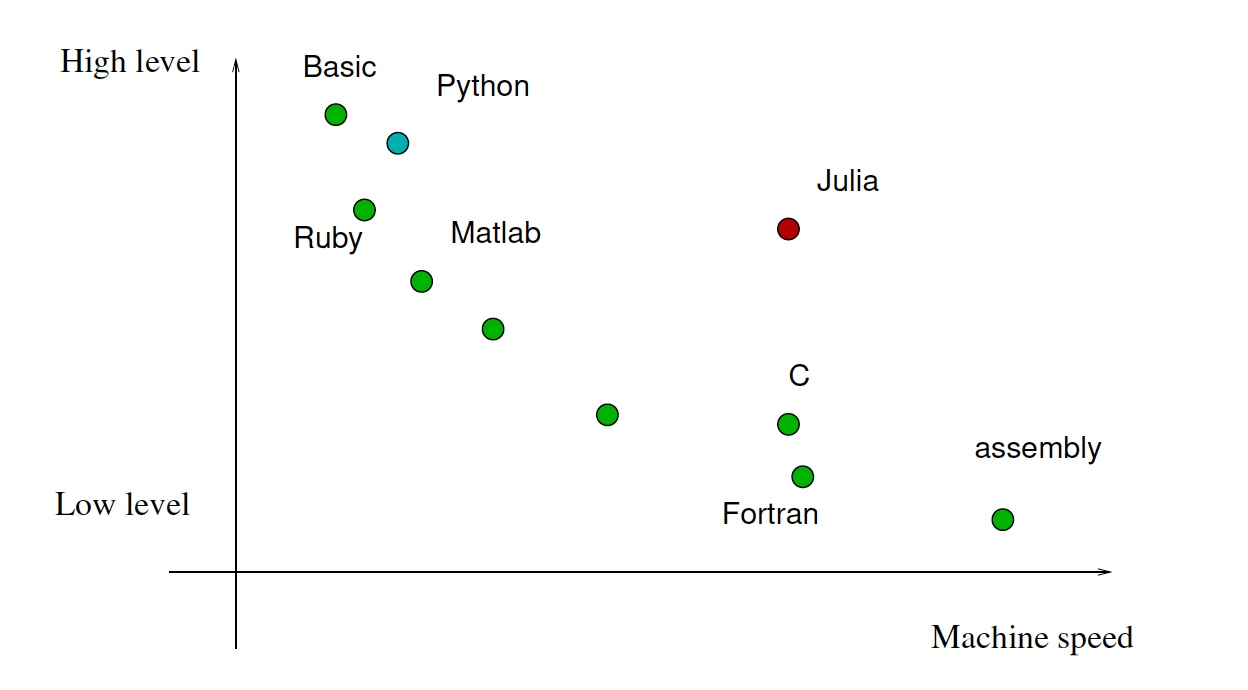
\includegraphics[width=\textwidth]{languages_shifted.jpeg}
  \end{figure}
\end{frame}

\begin{frame}
  \frametitle{A Horse Race}

  \boldblue{Task:}
  \vspace{1em}
  \begin{enumerate}
    \item Compute $X_1, X_2, \dots, X_n$ according to $X_{t+1} = \beta + \alpha X_{t} + W_{t+1}$, where $W_t \sim N(0,1)$
    \item Calculate and return $ \frac{1}{n} \sum_{t=1}^n X_t $
  \end{enumerate}

  \vspace{1em}
  Where $n = 10^7$

\end{frame}

\section{Getting Started With Julia}
\begin{frame}
  \frametitle{Julia Overview}

  High-level, open-source, scientific computing language \\

  \vspace{1em}
  \boldblue{Strengths}
  \begin{itemize}
    \item High productivity
    \item And high performance!
  \end{itemize}

  \pause
  \vspace{1em}
  \boldblue{Potential Negatives}
  \begin{itemize}
    \item Still under rapid development (will slow w/ v1.0)
    \item Lots of advanced features either out there or in development: rabbit holes abound
  \end{itemize}

\end{frame}

\begin{frame}
  \frametitle{Why (free and) Open Source?}

  \begin{itemize}
    \setlength\itemsep{1em}

    \item Reproducibility with minimal headache:

      \begin{quote}
        Let's be clear: the work of science has nothing whatever
        to do with consensus. Consensus is the business of
        politics. Science, on the contrary, requires only one
        investigator who happens to be right, which means that
        he or she has results that are veriable by reference to
        the real world. In science consensus is irrelevant. What is
        relevant is reproducible results.

        \hspace{1em} - Michael Crichton
      \end{quote}
    \pause

    \item Free! Don't rely on expensive licenses
  \end{itemize}
\end{frame}

\begin{frame}
  \frametitle{Interacting with Julia}

  \boldblue{Options:}

  \begin{itemize}
    \setlength\itemsep{1em}
    \item REPL + text editor (Atom, Sublime, Emacs, etc)
      \begin{itemize}
        \item Minimal difference from language to language
        \item Customize your text editor as much as you want
      \end{itemize}
      \pause
    \item IDEs like Juno
      \begin{itemize}
        \item Mouse support: buttons, etc
        \item Possibly most familiar for MATLAB IDE users
      \end{itemize}
      \pause
    \item Jupyter notebooks
  \end{itemize}
\end{frame}

\begin{frame}
  \frametitle{Jupyter Notebooks}

  Browser-based front-end for Python, Julia, R, and increasingly more

  \vspace{1em}
  \begin{itemize}
    \item Easy to run in the cloud or on servers
    \item Allows for rich text and graphics - nice for presenting notes alongside computation
  \end{itemize}
  \vspace{1em}
  Examples: \href{http://notebooks.quantecon.org/}{http://notebooks.quantecon.org/}

  \pause
  \vspace{1em}
  Let's try one!
\end{frame}

\end{document}
